% ----- INPUT
\newcommand{\fcimagew}{0.45\textwidth}
\newcommand{\fcimageh}{\fcimagew}

% to shift for ticks
\newcommand{\fcshiftx}{1.3em}
\newcommand{\fcshifty}{1em}

% to shift to the middle from kinda the middle
\newcommand{\fcmidshiftx}{0.5em}
\newcommand{\fcmidshifty}{0.4em}

%
\newcommand{\fchormid}{0.5 * \fcimagew}
\newcommand{\fcvermid}{0.5 * \fcimageh}



\begin{tikzpicture}[
        arr/.style = { -{Stealth[ ]} },
        bluearrow/.style = {arr, draw=third-color, fill=third-color, thick},
        blackarrow/.style = {arr, ultra thick},
    ]
    
    \begin{scope}

        \node[
            shift={(\fcmidshiftx, -\fcshifty)}
        ] at (\fchormid, 0) {{ \small Current}};
        
        \node[
            shift={(-\fcshiftx, \fcmidshifty)},
            rotate=90
        ] at (0, \fcvermid) {{\small Frequency}};

        
        % \node[shift={(\apwest, \apshifth)}, anchor=west] at (0, \appeakh) {peak};
        
    \end{scope}
    
    \begin{scope}
        \node[anchor=south west,inner sep=0] at (0,0) {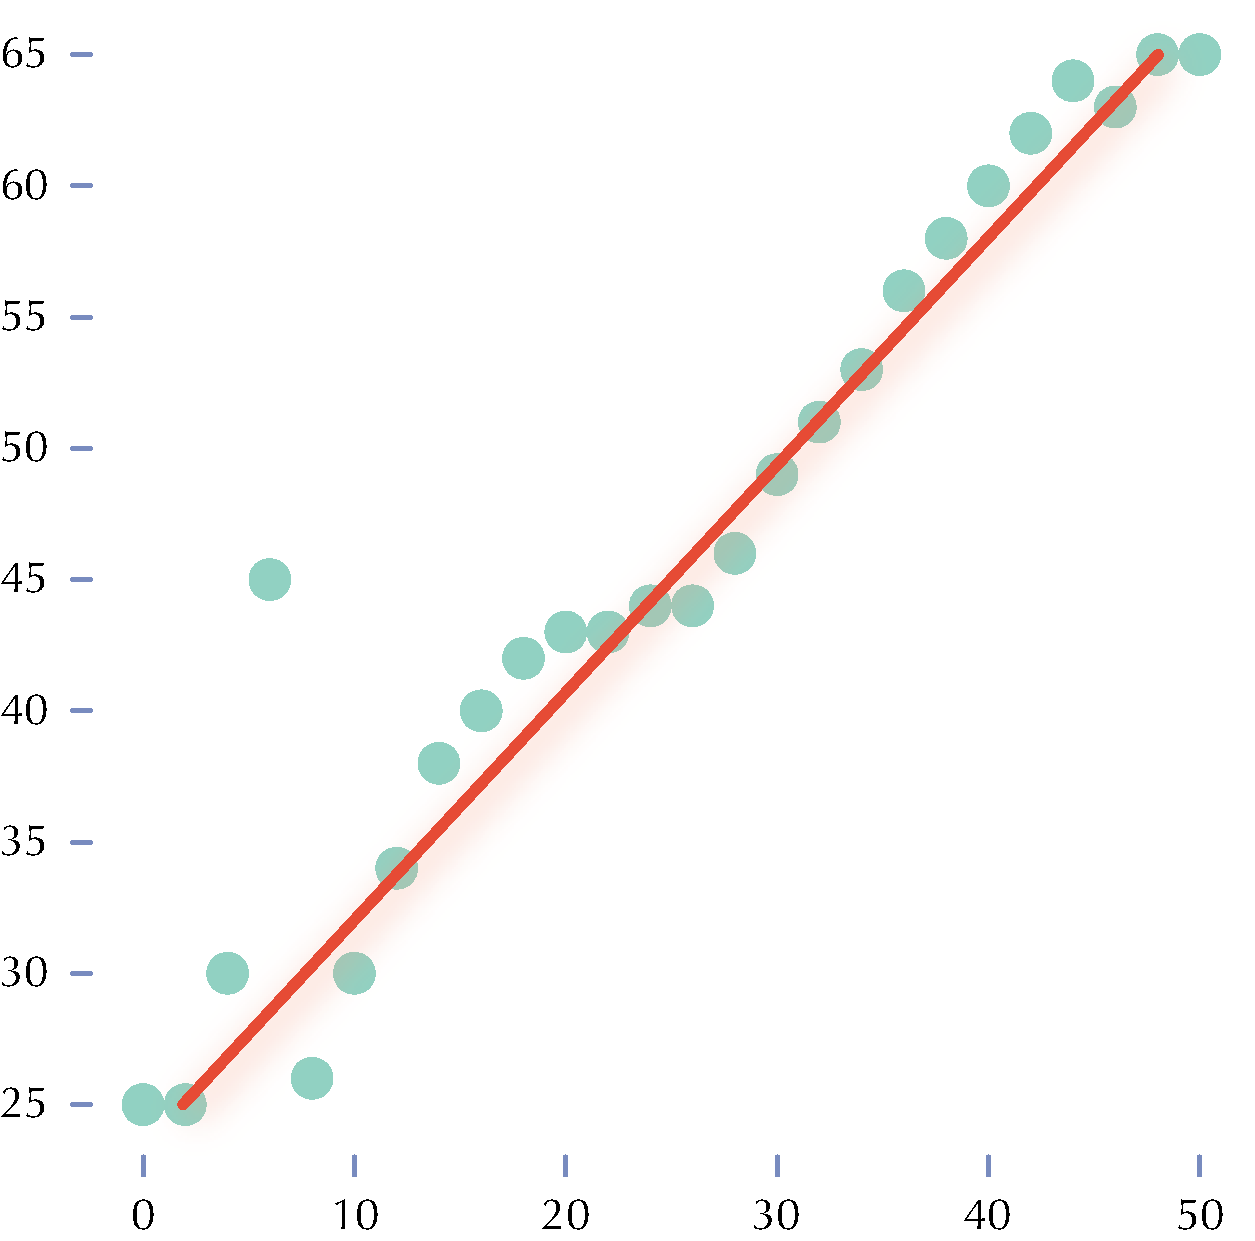
\includegraphics[width=\fcimagew]{src/assets/images/f-c-relationship.pdf}};
    \end{scope}
        
\end{tikzpicture}